\documentclass[paper=letter, fontsize=14pt]{scrartcl} 


\usepackage[utf8]{inputenc}
\usepackage{color}
\usepackage{hyperref}
\usepackage{graphicx}
\usepackage{epsfig}
\usepackage{multirow}
\usepackage{colortbl}
\usepackage[table]{xcolor}
\usepackage{fancyhdr}
\usepackage{graphicx}
\usepackage{graphicx}
\usepackage{verbatim}
\usepackage{pictex}  
\usepackage{multimedia}
\usepackage{listings}
\usepackage{vmargin}
\usepackage{xcolor,colortbl}
\usepackage[spanish]{babel} % language/hyphenation
\usepackage{amsmath,amsfonts,amsthm} % Math packages
\usepackage{amsbsy}
\usepackage{amssymb}
\usepackage{fancyvrb}
\usepackage{sectsty} % Allows customizing section commands
\allsectionsfont{\centering \normalfont\scshape} % Make all sections centered, the default font and small caps

\usepackage{fancyhdr} % Custom headers and footers
\pagestyle{fancyplain} % Makes all pages in the document conform to the custom headers and footers
\fancyhead{} % No page header - if you want one, create it in the same way as the footers below
\fancyfoot[L]{} % Empty left footer
\fancyfoot[C]{} % Empty center footer
\fancyfoot[R]{\thepage} % Page numbering for right footer
\renewcommand{\headrulewidth}{0pt} % Remove header underlines
\renewcommand{\footrulewidth}{0pt} % Remove footer underlines
\setlength{\headheight}{13.6pt} % Customize the height of the header

\numberwithin{equation}{section} % Number equations within sections (i.e. 1.1, 1.2, 2.1, 2.2 instead of 1, 2, 3, 4)
\numberwithin{figure}{section} % Number figures within sections (i.e. 1.1, 1.2, 2.1, 2.2 instead of 1, 2, 3, 4)
\numberwithin{table}{section} % Number tables within sections (i.e. 1.1, 1.2, 2.1, 2.2 instead of 1, 2, 3, 4)
\setpapersize{A4}
\setmargins{2.5cm}       % margen izquierdo
{2.4cm}                        % margen superior
{16.5cm}                      % anchura del texto
{23.42cm}                    % altura del texto
{10pt}                           % altura de los encabezados
{1cm}                           % espacio entre el texto y los encabezados
{0pt}                             % altura del pie de página
{2cm}                           % espacio entre el texto y el pie de página

\setlength\parindent{0pt} % Removes all indentation from paragraphs - comment this line for an assignment with lots of text

\newcommand{\horrule}[1]{\rule{\linewidth}{#1}} % Create horizontal rule command with 1 argument of height

\title{	
\normalfont \normalsize 
\textsc{Centro de Investigaci\'on en Matem\'aticas (CIMAT). Unidad Monterrey} 
\\ [25pt] 
\horrule{0.5pt} \\[0.4cm] % Thin top horizontal rule
\huge \textbf{Tracy Widom en modelos multivariados}\\ 
\horrule{2pt} \\[0.5cm] % Thick bottom horizontal rule
}

\author{Ricardo Cruz} % Your name

\date{\normalsize\today} % Today's date or a custom date


\rhead{\begin{picture}(0,0) \put(-56.7,-50){
\includegraphics[width=20mm]{cimat.png}} \end{picture}}
\renewcommand{\headrulewidth}{0.5pt}

\pagestyle{fancy}

\begin{document}
\lstdefinestyle{customc}{
  belowcaptionskip=1\baselineskip,
  basicstyle=\footnotesize, 
  frame=lrtb,
  breaklines=true,
  %frame=L,
  %xleftmargin=\parindent,
  language=C,
  showstringspaces=false,
  basicstyle=\footnotesize\ttfamily,
  keywordstyle=\bfseries\color{green!40!black},
  commentstyle=\itshape\color{red!40!black},
  identifierstyle=\color{blue},
  stringstyle=\color{purple},
}

\lstset{breakatwhitespace=true,
  basicstyle=\footnotesize, 
  commentstyle=\color{green},
  keywordstyle=\color{blue},
  stringstyle=\color{purple},
  language=C++,
  columns=fullflexible,
  keepspaces=true,
  breaklines=true,
  tabsize=3, 
  showstringspaces=false,
  extendedchars=true}

\lstset{ %
  language=R,    
  basicstyle=\footnotesize, 
  numbers=left,             
  numberstyle=\tiny\color{gray}, 
  stepnumber=1,              
  numbersep=5pt,             
  backgroundcolor=\color{white},
  showspaces=false,             
  showstringspaces=false,       
  showtabs=false,               
  frame=single,                 
  rulecolor=\color{black},      
  tabsize=2,                  
  captionpos=b,               
  breaklines=true,            
  breakatwhitespace=false,    
  title=\lstname,             
  keywordstyle=\color{blue},  
  commentstyle=\color{dkgreen},
  stringstyle=\color{mauve},   
  escapeinside={\%*}{*)},      
  morekeywords={*,...}         
} 


\maketitle % Print the title


\pagebreak

\textbf{Ejercicio 1:}\\
El ejercicio 1 se plantea el modelo general spiked. El cual realiza una corrección al modelo APT para los valores propios estimados.\\

La figura 1 y 2 muestran el modelo APT sin y con el modelo spiked respectivamente.\\

De manera general, la corrección es multiplicar por un factor mayor a 1, lo cual implica valores propios más grandes a comparación de cuando no se ocupo el modelo spiked. \\

La principal consecuencia de esto es tener valores propios simulados más cercanos a los valores teóricos (lineas verdes en los gráficos).

\begin{figure}[h]
\centering
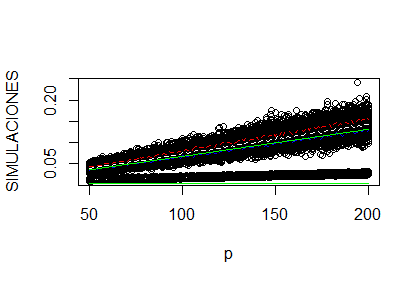
\includegraphics[scale=1]{i1.png} 
\caption{modelo APT}
\end{figure}

\begin{figure}[h]
\centering
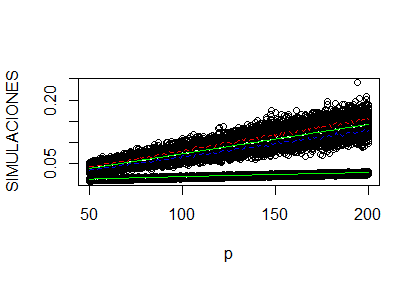
\includegraphics[scale=1]{i2.png} 
\caption{modelo APT con el modelo spiked}
\end{figure}


\pagebreak

\textbf{Ejercicio 2:}\\
El ejercicio 2 busca aplicar Tracy Widom en MANOVA al comparar los resultados del ejercicio 6.17 de Rencher (2002).\\

En este ejercicio se tiene que son 48 observaciones de 6 categorias y 4 variables. \\

El valor de $\theta_{obs}$ es .652, por lo tanto el valor propio mayor es 1.87\\

Aplicando Tracy Widom, a un nivel de significancia de .05, se tiene que $\theta_{TW}=.38$. Lo cual implica que el valor propio más grande sería de .62\\

Por lo tanto se rechaza la hipotesis nula, pues bajo esta, el valor propio más grande excede el que se plantea con Tracy Widom.

\pagebreak


\end{document}
